\subsection{Isosurface extraction}\label{sec:isocontour}

\begin{figure*}[h]
\centering
\subcaptionbox{\em pressure, isovalue=0.2}
{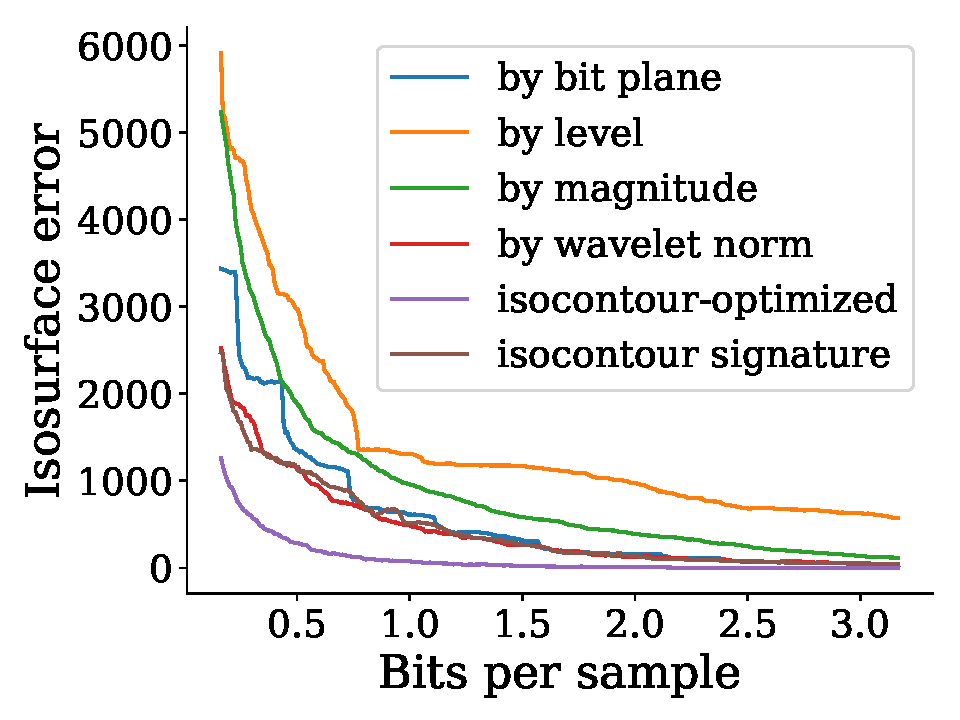
\includegraphics[width=0.24\linewidth]{isocontour/isocontour-optimized-pressure}}
\subcaptionbox{\em kingsnake, isovalue=106}
{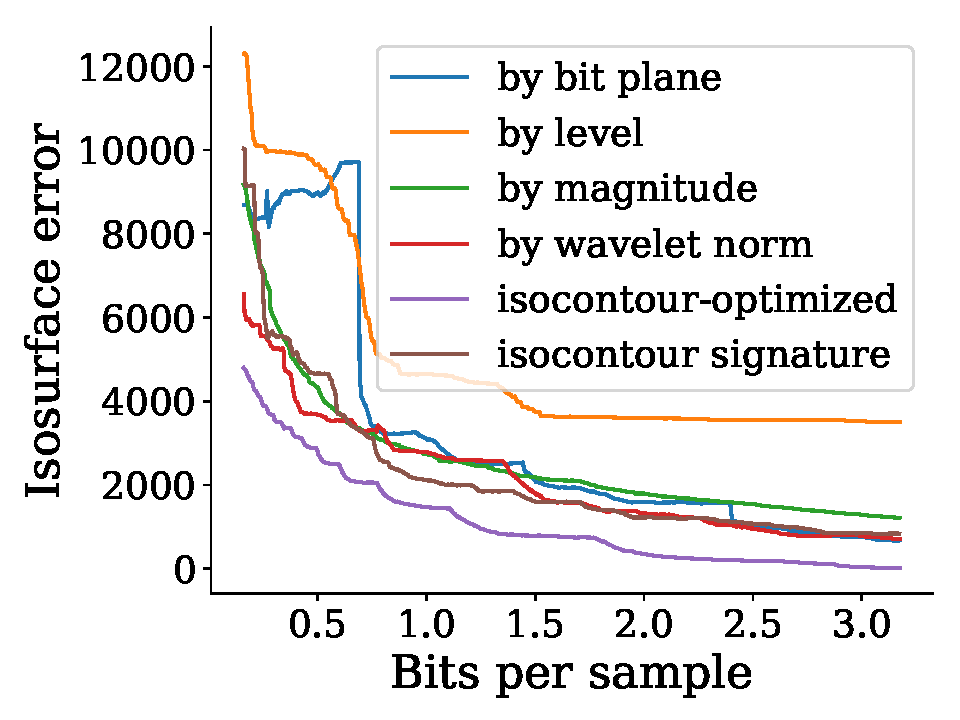
\includegraphics[width=0.24\linewidth]{isocontour/isocontour-optimized-kingsnake}}
\subcaptionbox{\em plasma, isovalue=2}
{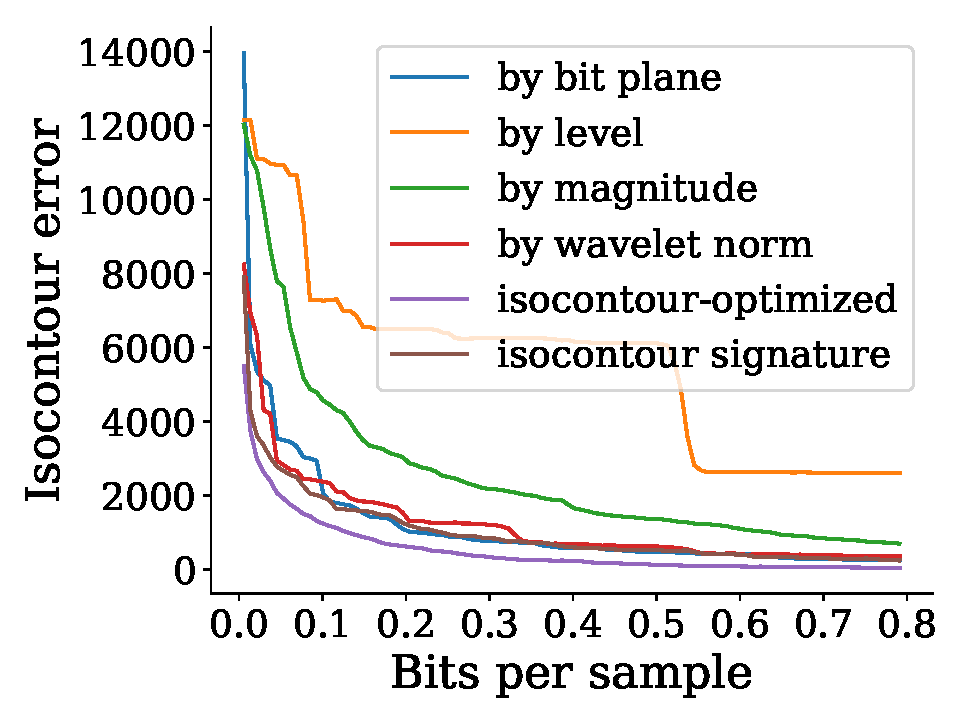
\includegraphics[width=0.24\linewidth]{isocontour/isocontour-optimized-plasma}}
\subcaptionbox{\em turbulence, isovalue=2}
{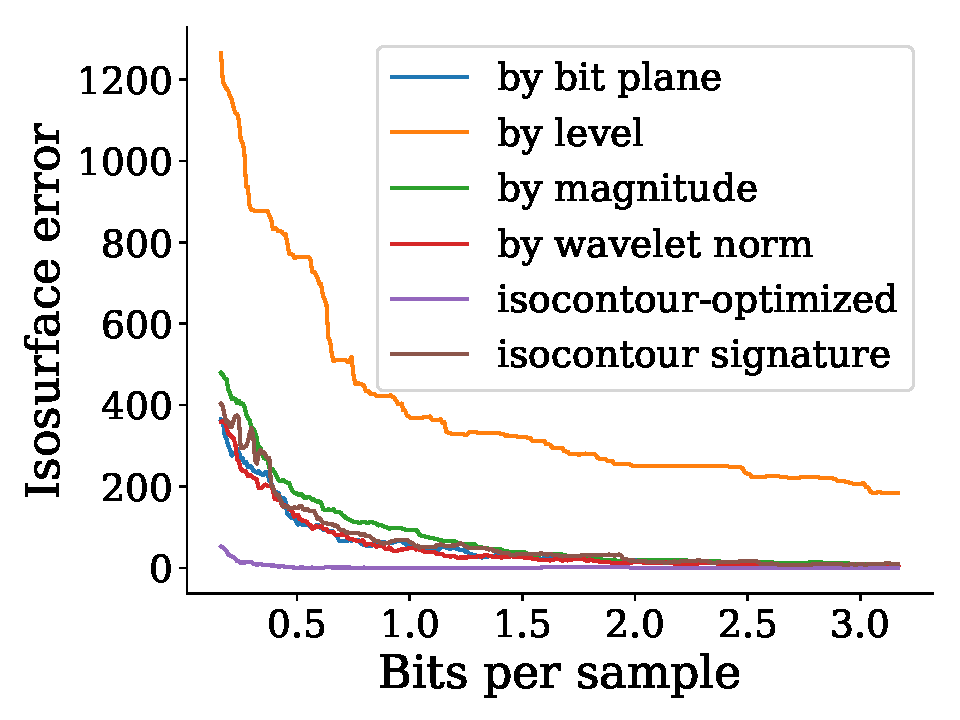
\includegraphics[width=0.24\linewidth]{isocontour/isocontour-optimized-turbulence}}
\caption{Comparison of isosurface errors among streams. Plots are truncated to highlight differences
without hiding important trends. In all cases, \slvl performs significantly worse than the rest.
\swav outperforms \sbit for \emph{pressure} and \emph{kingsnake}, but not for \emph{plasma} and \emph{turbulence}.}\label{fig:isocontour-plots}
\vspace{1em}

\centering
\subcaptionbox{\emph{by level} ($s_{lvl}$)}
{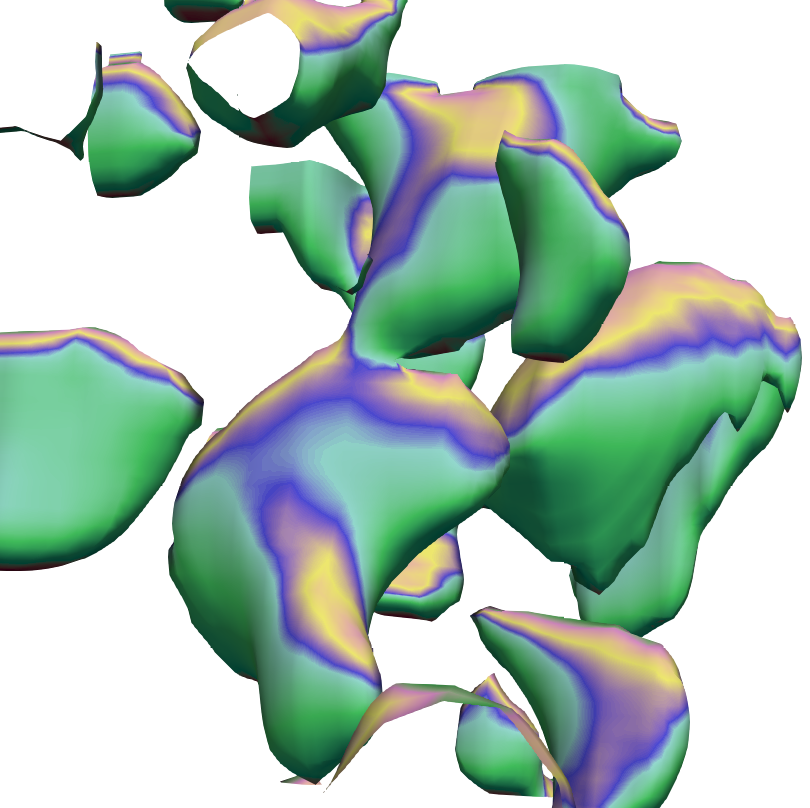
\includegraphics[width=0.16\linewidth]{isocontour/isocontour-level}}
\subcaptionbox{\emph{by bit plane} ($s_{bit}$)}
{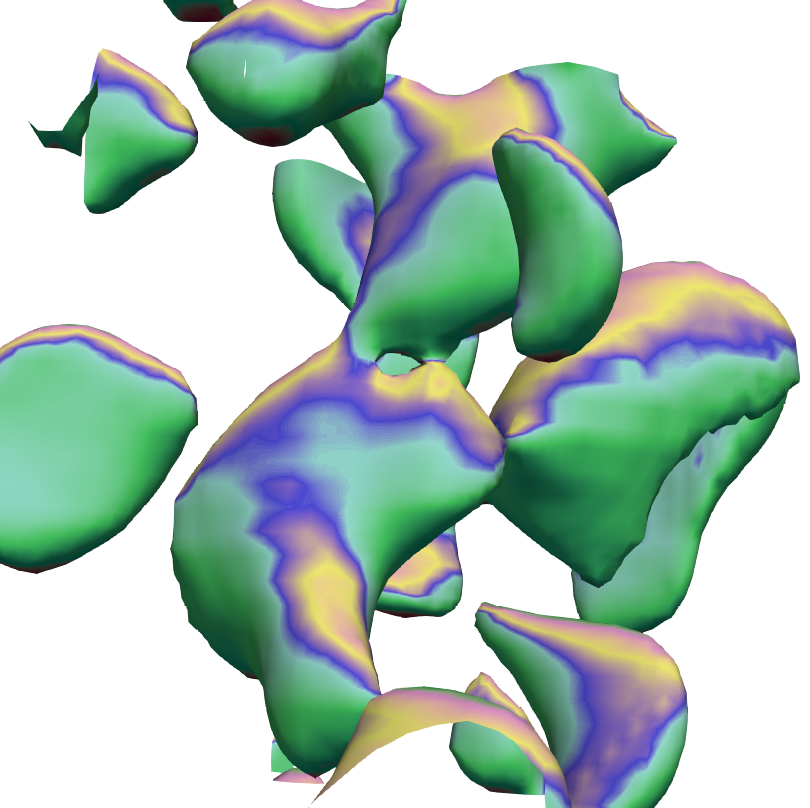
\includegraphics[width=0.16\linewidth]{isocontour/isocontour-bit-plane}}
\subcaptionbox{\emph{by wavelet norm} ($s_{wav}$)}
{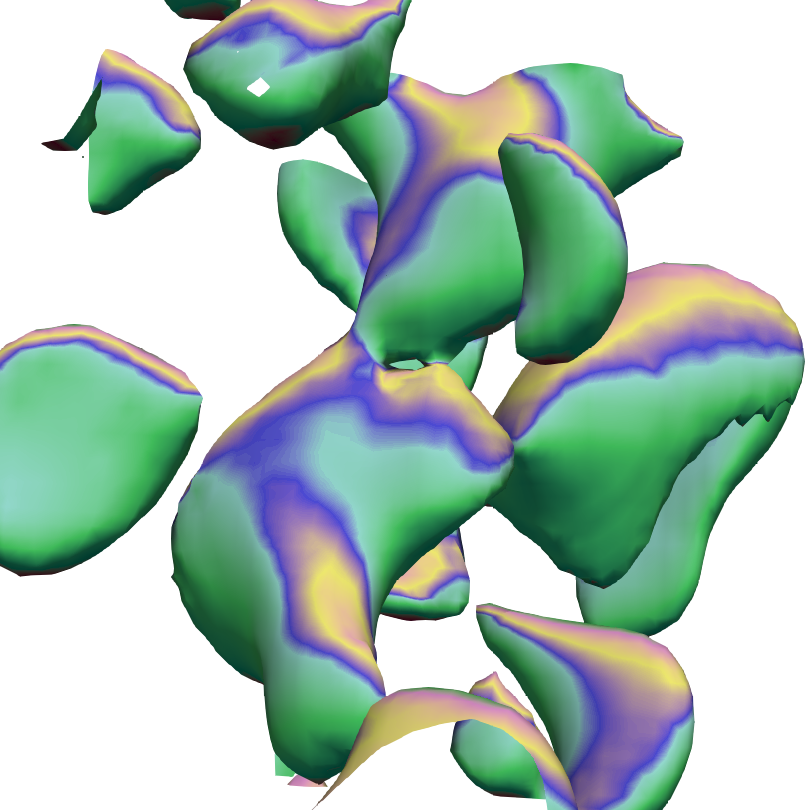
\includegraphics[width=0.16\linewidth]{isocontour/isocontour-wavelet-norm}}
\subcaptionbox{\emph{by magnitude} ($s_{mag}$)}
{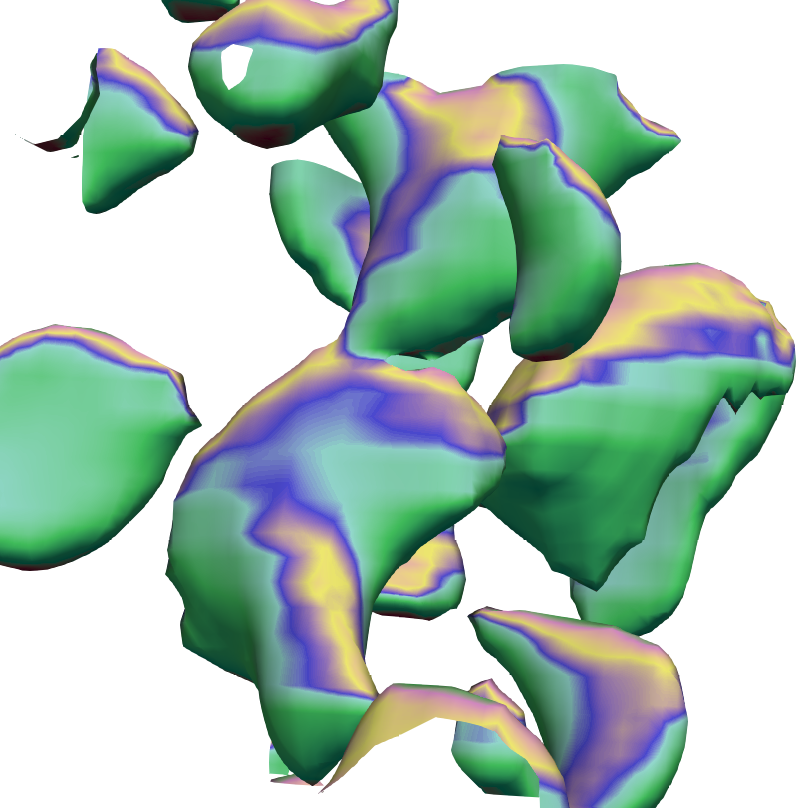
\includegraphics[width=0.16\linewidth]{isocontour/isocontour-magnitude}}
\subcaptionbox{\emph{by signature} ($s_{iso-sig}$)}
{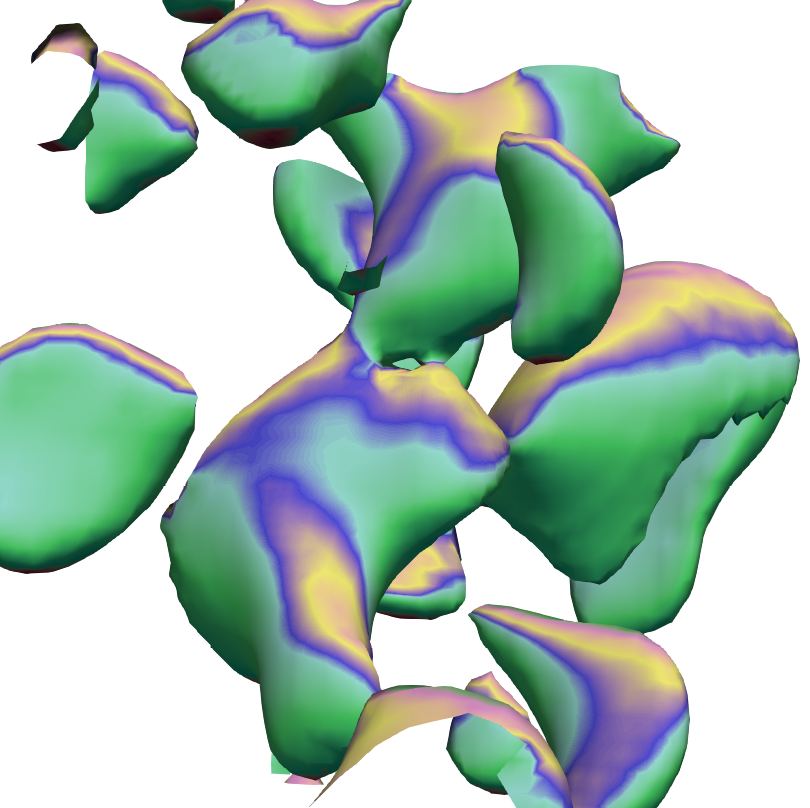
\includegraphics[width=0.16\linewidth]{isocontour/isocontour-signature}}
\subcaptionbox{\emph{ground truth}}
{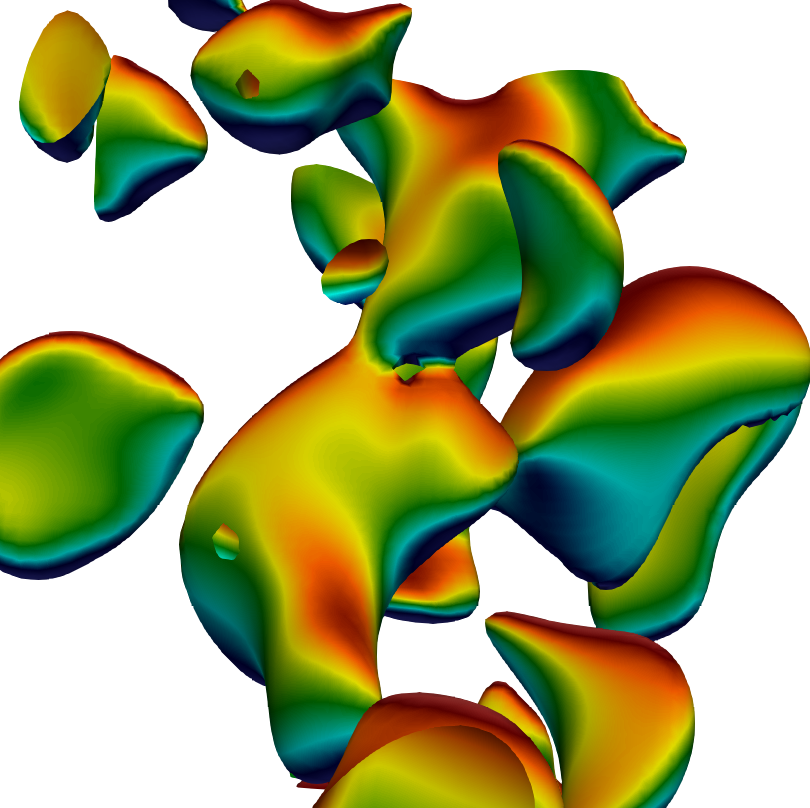
\includegraphics[width=0.16\linewidth]{isocontour/isocontour-groundtruth}}
\caption{Rendering of isosurfaces at isovalue of 0.2, at 0.7 bps, for the \emph{pressure} data set.
The surfaces are colored by the $x$-component of the normal vector at each point. \swav and
\sisg produce surfaces that are closest to the reference, followed by \sbit, \smag, and \slvl.}
\label{fig:isocontour-surfaces-pressure}
\end{figure*}

\begin{figure}[h]
\centering
\subcaptionbox{\emph{by bit plane} (\sbit)}
{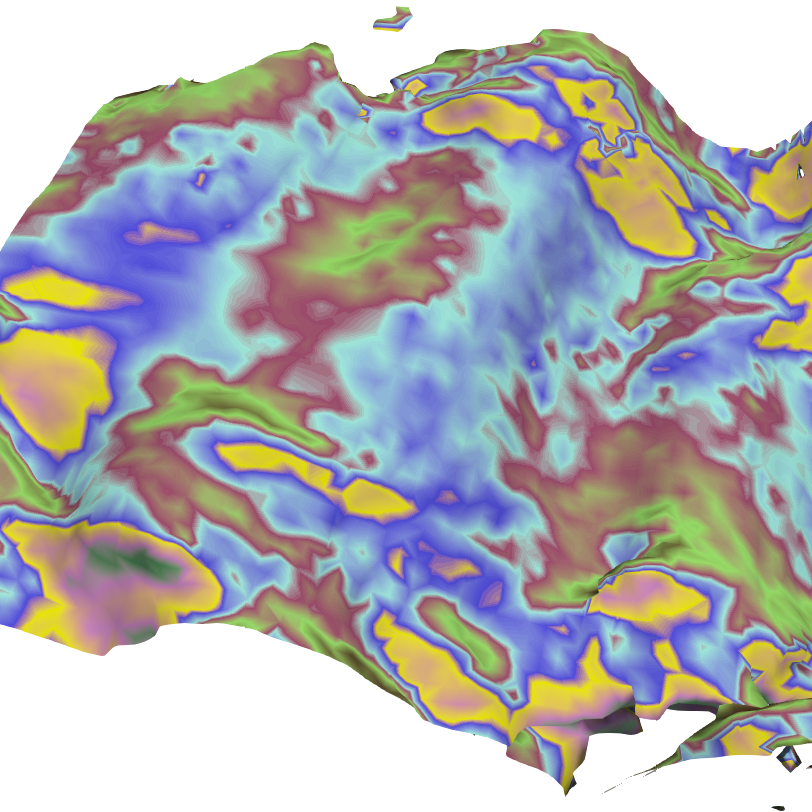
\includegraphics[width=0.32\linewidth]{isocontour/isocontour2-bit-plane}}
\subcaptionbox{\emph{by wavelet norm} (\swav)}
{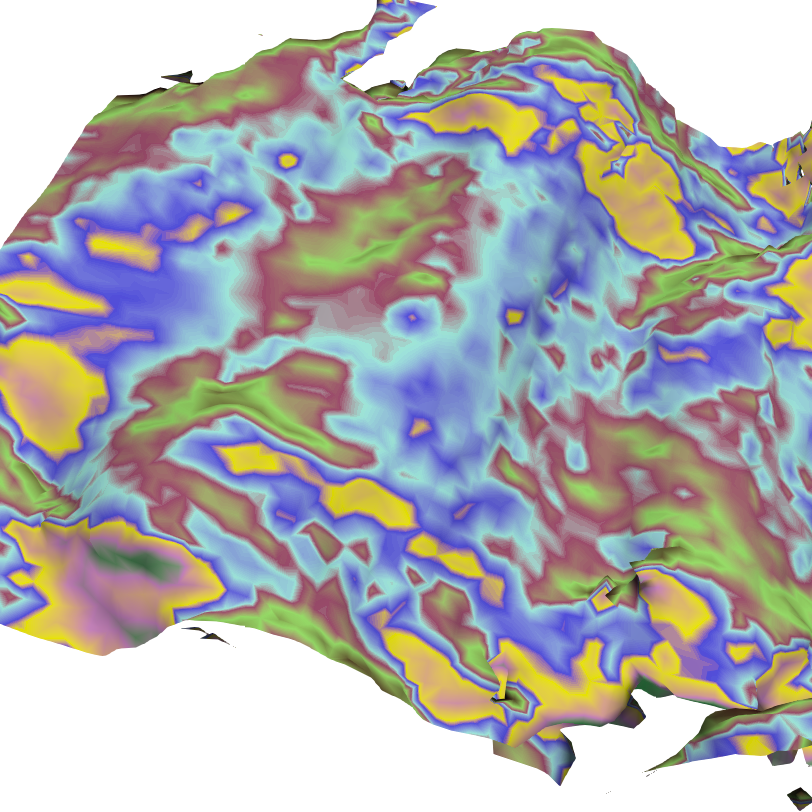
\includegraphics[width=0.32\linewidth]{isocontour/isocontour2-wavelet-norm}}
\subcaptionbox{\emph{ground truth}}
{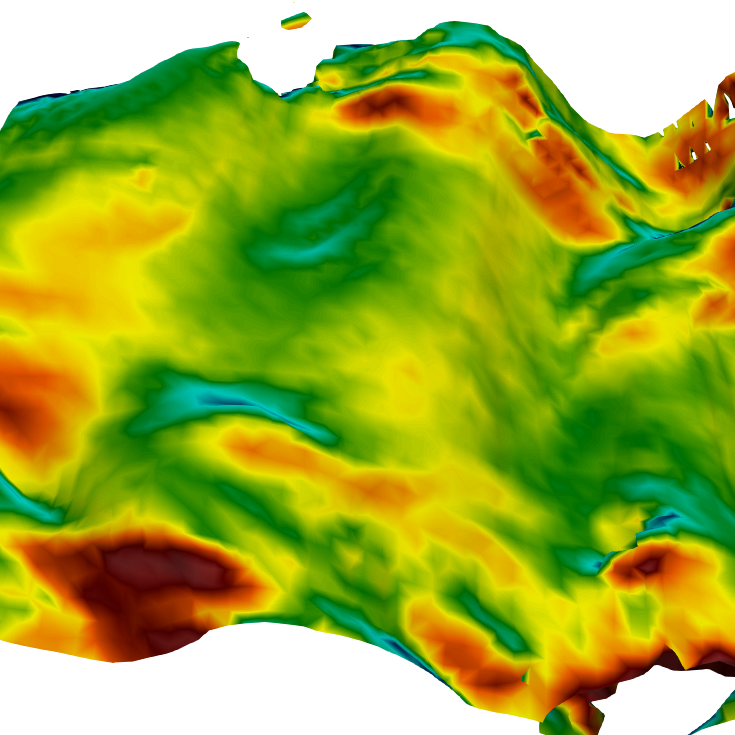
\includegraphics[width=0.32\linewidth]{isocontour/isocontour2-groundtruth}}
\caption{\emph{plasma}'s isosurface reconstructed at 0.5 bps. The surfaces are colored by the
$x$-component of the normal vectors. The reconstruction by \sbit is closer to the reference (compare
e.g., yellow features and green features).}
\label{fig:isocontour-surfaces-plasma}
\end{figure}

Studying isosurfaces of a given function is an essential task in many visualization and analysis
pipelines, as they can highlight features of interest. For example, in combustion simulations,
separation of burning and extinguished regions can be performed by extracting isosurfaces of OH
concentration.

Several sophisticated metrics exist that may be used to measure error in isosurface extraction,
focusing on different characteristics, including geometric~\cite{verifiable-isosurface} and
topological~\cite{topology-verification-isosurface} properties. Commonly used Hausdorff distance is
another choice, but is not very robust as it varies drastically with minor changes in the surfaces.
Since isosurfaces partition the domain into ``inside'' and ``outside'' regions, we opt for a simpler
error metric that assumes nothing about the shape of the isosurfaces, but simply counts
misclassified voxels. However, if the error caused by discarding a packet is of subvoxel resolution,
such a metric does not capture the importance of that packet, causing~\Cref{alg:greedy} to produce a
suboptimal \siop. Therefore, we add the relative difference in surface areas ($|A_1-A_2|/|A_1|$) to
the error term. The normalization reduces the range of this term to $[0, 1]$, so that when the
number of misclassified voxels is less than one, the subvoxel error is instead captured by this
relative difference in surface areas.

With the error metric defined, we can compute a data-dependent stream optimized for this metric
(\siop) and a stream based on its signature (\sisg) using~\Cref{alg:greedy}
and~\Cref{alg:signature}. \Cref{fig:isocontour-plots} compares the performances of these two
streams, along with \sbit, \slvl, \swav, and \smag. As can be noticed, both \slvl performs poorly,
indicating that isosurface extraction favors resolution over precision. \emph{plasma} is the only
data set where \sbit outperforms \swav.

For \emph{plasma}, the isosurface is extracted from a region with a low gradient, which means the
surface is very sensitive to low-ordered bits (i.e., a slight change in values moves the isosurface
by a larger distance). For this reason, \swav initially performs better (below 0.2 bps), as it
streams more precision bits. As \sbit acquires enough precision, however, it starts to resolve the
fine-scale geometry of the surface better than \swav
(from~\autoref{fig:bit-plane-vs-wavelet-norm-gradient} in~\Cref{sec:gradient}, we learn that \swav
tends to reconstruct a smoother function everywhere).

\Cref{fig:isocontour-surfaces-plasma} shows the renderings of the surfaces reconstructed by \sbit
and \swav at 0.5 bps, which confirm that \sbit is able to preserve better the fine-scale featureas
on the surface. For the \emph{turbulence} field, the isosurface is extracted from a high-gradient
region; thus precision bits matter less, and \sbit outperforms \swav from the beginning. \sbit also
outperforms \sisg in this case, because local signatures coming from regions where the isosurface
does not intersect can dilute those coming from regions where it does. This phenomenon makes the
signature less useful for tasks that involve localization in the spatial domain, such as isosurface
extraction. Here, it happens in various degrees for every data set but it is especially relevant in
the case of \emph{turbulence}, since the surface is confined to very small regions of the whole
volume.

For a typical isosurface that is relatively smooth and is not confined to small regions, such as
\emph{pressure} with an isovalue of 0.2, \swav typically outperforms \sbit
(see~\Cref{fig:isocontour-surfaces-pressure})\pavol{Fig 14 is after Fig 15 in text}. This figure
renders the isosurfaces reconstructed at 0.7 bps for all streams. In terms of the quality of the
reconstructed surfaces, $\sisg \approx \swav > \sbit > \smag > \slvl$, which agrees with the curves
in~\autoref{fig:isocontour-plots}. For isosurface extraction, \swav seems to be the only stream ---
among the data-independent ones --- that consistently works well in all cases.
